%! TeX program = lualatex
\documentclass[a4paper,12pt,article]{memoir}

% TeX root=../main.tex

\settrimmedsize{\stockheight}{\stockwidth}{*}
\settypeblocksize{220mm}{130mm}{*}
\setlrmargins{*}{*}{1.7}
\setulmargins{30mm}{*}{*}
\setmarginnotes{20pt}{100pt}{10pt}
\checkandfixthelayout%

% \setsidefeet{\marginparsep}{\marginparwidth}%
% {0.8\onelineskip}{0pt}%
% {\normalfont\footnotesize}{\textheight}%
\setsidecaps{\marginparsep}{\marginparwidth}
\setlength{\footmarkwidth}{0.5em}
\setlength{\footmarksep}{0em}
\setlength{\footparindent}{0em}
\footmarkstyle{\textsuperscript{#1}\hspace{0.5em}}

\makeoddfoot{plain}{}{}{\thepage}
\makeevenfoot{plain}{\thepage}{}{}
\makepagestyle{ruled}
\makeevenfoot{ruled}{\thepage}{}{} % page numbers at the outside
\makeoddfoot{ruled}{}{}{\thepage}
\makeheadrule{ruled}{\textwidth}{0.75pt}
\makeevenhead{ruled}{\scshape\leftmark}{}{}
\makeoddhead{ruled}{}{}{\scshape\rightmark}
\makepsmarks{ruled}{%
	\nouppercaseheads%
	\createmark{chapter}{left}{shownumber}{\scshape}{.\space}
	\createmark{part}{right}{shownumber}{}{.\space}
	\createmark{section}{right}{shownumber}{}{.\space}
	\createmark{subsection}{right}{shownumber}{}{.\space}
	\createplainmark{toc}{both}{\contentsname}
	\createplainmark{lof}{both}{\listfigurename}
	\createplainmark{lot}{both}{\listtablename}
	\createplainmark{bib}{both}{\bibname}
	\createplainmark{index}{both}{\indexname}
	\createplainmark{glossary}{both}{\glossaryname}
}

% decorando divisões
\setsecnumdepth{subsection}
\setcounter{tocdepth}{3}
\newcommand\chap[1]{%
	\chapter*[#1]{#1}%
	\addcontentsline{toc}{chapter}{#1}}


% paleta de cores
\usepackage{xcolor}
\definecolor{green}{rgb}{16,87,87} % rgb(16,87,87)
\definecolor{red}{rgb}{193, 11, 105} % rgb(193, 11, 105)
\definecolor{yellow}{rgb}{218,222,104} % rgb(218,222,104)
\definecolor{pink}{rgb}{243,179,145} % rgb(243,179,145)
\definecolor{blue}{rgb}{161,184,206} % rgb(161,184,206)

\usepackage[tracking=true]{microtype}

\usepackage{scalefnt}


\usepackage[normalem]{ulem}
\usepackage{paralist}
\usepackage{graphicx}
\usepackage{subcaption}
\usepackage{linguex}
\usepackage{multicol}
\usepackage{tabto}

\usepackage{hyperref}
\hypersetup{%
	colorlinks=true, % false: boxed links; true: colored links
	linkcolor=green,  % color of internal links
	citecolor=green,  % color of links to bibliography
	filecolor=pink,  % color of file links
	urlcolor=green,
}
% Configurações para o autoref
\renewcommand{\figureautorefname}{Figura}
\renewcommand{\tableautorefname}{Tabela}
\renewcommand{\sectionautorefname}{Seção}
\renewcommand{\chapterautorefname}{Capítulo}
\renewcommand{\subsectionautorefname}{Subseção}


\directlua{dofile('./utils/pie.lua')}
\newcommand{\hittitetrans}[1]{%
  \directlua{hittite_transcription("#1")}}
\newcommand{\luwiantrans}[1]{%
  \directlua{luwian_transcription("#1")}}
\newcommand{\pietrans}[1]{%
  \directlua{pie_transcription("#1")}}

\newcommand{\Prep}{{\footnotesize\textsc{Prep.}}}
\newcommand{\Det}{{\footnotesize\textsc{Det.}}}
\newcommand{\Clt}{{\footnotesize\textsc{Clt.}}}
\newcommand{\Nom}{{\footnotesize\textsc{Nom.}}}
\newcommand{\Acu}{{\footnotesize\textsc{Acu.}}}
\newcommand{\Dat}{{\footnotesize\textsc{Dat.}}}
\newcommand{\Gen}{{\footnotesize\textsc{Gen.}}}
\newcommand{\Abl}{{\footnotesize\textsc{Abl.}}}
\newcommand{\Sg}{{\footnotesize\textsc{Sg.}}}
\newcommand{\Pl}{{\footnotesize\textsc{Pl.}}}
\newcommand{\Com}{{\footnotesize\textsc{Com.}}}
\newcommand{\Neut}{{\footnotesize\textsc{Neut.}}}
\newcommand{\Rel}{{\footnotesize\textsc{Rel.}}}
\newcommand{\Conj}{{\footnotesize\textsc{Conj.}}}
\newcommand{\Pret}{{\footnotesize\textsc{Pret.}}}
\newcommand{\Pro}{{\footnotesize\textsc{Pro.}}}
\newcommand{\Refl}{{\footnotesize\textsc{Refl.}}}
\newcommand{\La}[1]{\textsc{l}.#1}
\newcommand{\logo}[1]{\textnormal{#1}}
\newcommand{\spac}{\textsuperscript{\textnormal{I}}}
\newcommand{\lmasc}{\textnormal{|}}
\newcommand{\luwmasc}{{\textsuperscript{𔖶}}}
\newcommand{\lbreak}{\hspace{2pt}\textnormal{||}\hspace{2pt}}
\newcommand{\parnumr}[2]{#1 \Roman{parcount}}
\newcommand{\parnuma}[2]{#1 \arabic{parcount}}
\newcounter{parcount}
\newenvironment{parnumbersa}[1][§]{%
   \par%
	 \everypar{\hangpara{3em}{1}\stepcounter{parcount} \textnormal{\normalsize\parnuma{#1}}
	 \tabto{2em}}%
}{}
\newenvironment{parnumbersr}[2][§]{%
   \par%
	 \everypar{\hangpara{3em}{1}\stepcounter{parcount} \textnormal{\normalsize\parnumr{#1}}
	 \tabto{2em}}%
}{}

\usepackage{csquotes}
\usepackage{fontspec}
\usepackage[main=brazil]{babel}
\defaultfontfeatures{Renderer=Harfbuzz}

\babelfont[brazil]{rm}[
	SmallCapsFont=Gentium Plus,
	SmallCapsFeatures={Letters=SmallCaps}]{Crimson Pro}
\babelfont[brazil]{sf}{Noto Sans}
\babelfont[brazil]{tt}[Scale=0.8]{Mononoki Nerd Font}

\babelfont[german]{rm}[
	SmallCapsFont=Gentium Plus,
	SmallCapsFeatures={Letters=SmallCaps}]{Crimson Pro}
\babelfont[brazil]{sf}{Noto Sans}
\babelfont[brazil]{tt}[Scale=0.8]{Mononoki Nerd Font}

\babelfont[english]{rm}[
	SmallCapsFont=Gentium Plus,
	SmallCapsFeatures={Letters=SmallCaps}]{Crimson Pro}
\babelfont[english]{sf}{Noto Sans}
\babelfont[english]{tt}[Scale=0.8]{Mononoki Nerd Font}

\babelfont[german]{rm}[
	SmallCapsFont=Gentium Plus,
	SmallCapsFeatures={Letters=SmallCaps}]{Crimson Pro}
\babelfont[german]{sf}{Noto Sans}
\babelfont[german]{tt}[Scale=0.8]{Mononoki Nerd Font}


\babelprovide[import, onchar=ids fonts letters]{ancientgreek}
\babelfont[ancientgreek]{rm}{Brill}
\babeltags{grc = ancientgreek}

\babelprovide[import]{hebrew}
\babelfont[hebrew]{rm}[Scale=0.8]{Ezra SIL}

\babelprovide[onchar=ids fonts]{luwian}
\babelfont[luwian]{rm}[
	SmallCapsFont=Gentium Plus,
Script=Anatolian Hieroglyphs]{Noto Sans Anatolian Hieroglyphs}
\babelfont[luwian]{sf}[
	SmallCapsFont=Gentium Plus,
Script=Anatolian Hieroglyphs]{Noto Sans Anatolian Hieroglyphs}
\babelcharproperty{`𔐀}{locale}{luwian}
\babelcharproperty{`𔐁}{locale}{luwian}
\babelcharproperty{`𔐂}{locale}{luwian}
\babelcharproperty{`𔐃}{locale}{luwian}
\babelcharproperty{`𔐄}{locale}{luwian}
\babelcharproperty{`𔐅}{locale}{luwian}
\babelcharproperty{`𔐆}{locale}{luwian}
\babelcharproperty{`𔐇}{locale}{luwian}
\babelcharproperty{`𔐈}{locale}{luwian}
\babelcharproperty{`𔐉}{locale}{luwian}
\babelcharproperty{`𔐊}{locale}{luwian}
\babelcharproperty{`𔐋}{locale}{luwian}
\babelcharproperty{`𔐌}{locale}{luwian}
\babelcharproperty{`𔐍}{locale}{luwian}
\babelcharproperty{`𔐎}{locale}{luwian}
\babelcharproperty{`𔐏}{locale}{luwian}
\babelcharproperty{`𔐐}{locale}{luwian}
\babelcharproperty{`𔐑}{locale}{luwian}
\babelcharproperty{`𔐒}{locale}{luwian}
\babelcharproperty{`𔐓}{locale}{luwian}
\babelcharproperty{`𔐔}{locale}{luwian}
\babelcharproperty{`𔐕}{locale}{luwian}
\babelcharproperty{`𔐖}{locale}{luwian}
\babelcharproperty{`𔐗}{locale}{luwian}
\babelcharproperty{`𔐘}{locale}{luwian}
\babelcharproperty{`𔐙}{locale}{luwian}
\babelcharproperty{`𔐚}{locale}{luwian}
\babelcharproperty{`𔐛}{locale}{luwian}
\babelcharproperty{`𔐜}{locale}{luwian}
\babelcharproperty{`𔐝}{locale}{luwian}
\babelcharproperty{`𔐞}{locale}{luwian}
\babelcharproperty{`𔐟}{locale}{luwian}
\babelcharproperty{`𔐠}{locale}{luwian}
\babelcharproperty{`𔐡}{locale}{luwian}
\babelcharproperty{`𔐢}{locale}{luwian}
\babelcharproperty{`𔐣}{locale}{luwian}
\babelcharproperty{`𔐤}{locale}{luwian}
\babelcharproperty{`𔐥}{locale}{luwian}
\babelcharproperty{`𔐦}{locale}{luwian}
\babelcharproperty{`𔐧}{locale}{luwian}
\babelcharproperty{`𔐨}{locale}{luwian}
\babelcharproperty{`𔐩}{locale}{luwian}
\babelcharproperty{`𔐪}{locale}{luwian}
\babelcharproperty{`𔐫}{locale}{luwian}
\babelcharproperty{`𔐬}{locale}{luwian}
\babelcharproperty{`𔐭}{locale}{luwian}
\babelcharproperty{`𔐮}{locale}{luwian}
\babelcharproperty{`𔐯}{locale}{luwian}
\babelcharproperty{`𔐰}{locale}{luwian}
\babelcharproperty{`𔐱}{locale}{luwian}
\babelcharproperty{`𔐲}{locale}{luwian}
\babelcharproperty{`𔐳}{locale}{luwian}
\babelcharproperty{`𔐴}{locale}{luwian}
\babelcharproperty{`𔐵}{locale}{luwian}
\babelcharproperty{`𔐶}{locale}{luwian}
\babelcharproperty{`𔐷}{locale}{luwian}
\babelcharproperty{`𔐸}{locale}{luwian}
\babelcharproperty{`𔐹}{locale}{luwian}
\babelcharproperty{`𔐺}{locale}{luwian}
\babelcharproperty{`𔐻}{locale}{luwian}
\babelcharproperty{`𔐼}{locale}{luwian}
\babelcharproperty{`𔐽}{locale}{luwian}
\babelcharproperty{`𔐾}{locale}{luwian}
\babelcharproperty{`𔐿}{locale}{luwian}
\babelcharproperty{`𔑀}{locale}{luwian}
\babelcharproperty{`𔑁}{locale}{luwian}
\babelcharproperty{`𔑂}{locale}{luwian}
\babelcharproperty{`𔑃}{locale}{luwian}
\babelcharproperty{`𔑄}{locale}{luwian}
\babelcharproperty{`𔑅}{locale}{luwian}
\babelcharproperty{`𔑆}{locale}{luwian}
\babelcharproperty{`𔑇}{locale}{luwian}
\babelcharproperty{`𔑈}{locale}{luwian}
\babelcharproperty{`𔑉}{locale}{luwian}
\babelcharproperty{`𔑊}{locale}{luwian}
\babelcharproperty{`𔑋}{locale}{luwian}
\babelcharproperty{`𔑌}{locale}{luwian}
\babelcharproperty{`𔑍}{locale}{luwian}
\babelcharproperty{`𔑎}{locale}{luwian}
\babelcharproperty{`𔑏}{locale}{luwian}
\babelcharproperty{`𔑐}{locale}{luwian}
\babelcharproperty{`𔑑}{locale}{luwian}
\babelcharproperty{`𔑒}{locale}{luwian}
\babelcharproperty{`𔑓}{locale}{luwian}
\babelcharproperty{`𔑔}{locale}{luwian}
\babelcharproperty{`𔑕}{locale}{luwian}
\babelcharproperty{`𔑖}{locale}{luwian}
\babelcharproperty{`𔑗}{locale}{luwian}
\babelcharproperty{`𔑘}{locale}{luwian}
\babelcharproperty{`𔑙}{locale}{luwian}
\babelcharproperty{`𔑚}{locale}{luwian}
\babelcharproperty{`𔑛}{locale}{luwian}
\babelcharproperty{`𔑜}{locale}{luwian}
\babelcharproperty{`𔑝}{locale}{luwian}
\babelcharproperty{`𔑞}{locale}{luwian}
\babelcharproperty{`𔑟}{locale}{luwian}
\babelcharproperty{`𔑠}{locale}{luwian}
\babelcharproperty{`𔑡}{locale}{luwian}
\babelcharproperty{`𔑢}{locale}{luwian}
\babelcharproperty{`𔑣}{locale}{luwian}
\babelcharproperty{`𔑤}{locale}{luwian}
\babelcharproperty{`𔑥}{locale}{luwian}
\babelcharproperty{`𔑦}{locale}{luwian}
\babelcharproperty{`𔑧}{locale}{luwian}
\babelcharproperty{`𔑨}{locale}{luwian}
\babelcharproperty{`𔑩}{locale}{luwian}
\babelcharproperty{`𔑪}{locale}{luwian}
\babelcharproperty{`𔑫}{locale}{luwian}
\babelcharproperty{`𔑬}{locale}{luwian}
\babelcharproperty{`𔑭}{locale}{luwian}
\babelcharproperty{`𔑮}{locale}{luwian}
\babelcharproperty{`𔑯}{locale}{luwian}
\babelcharproperty{`𔑰}{locale}{luwian}
\babelcharproperty{`𔑱}{locale}{luwian}
\babelcharproperty{`𔑲}{locale}{luwian}
\babelcharproperty{`𔑳}{locale}{luwian}
\babelcharproperty{`𔑴}{locale}{luwian}
\babelcharproperty{`𔑵}{locale}{luwian}
\babelcharproperty{`𔑶}{locale}{luwian}
\babelcharproperty{`𔑷}{locale}{luwian}
\babelcharproperty{`𔑸}{locale}{luwian}
\babelcharproperty{`𔑹}{locale}{luwian}
\babelcharproperty{`𔑺}{locale}{luwian}
\babelcharproperty{`𔑻}{locale}{luwian}
\babelcharproperty{`𔑼}{locale}{luwian}
\babelcharproperty{`𔑽}{locale}{luwian}
\babelcharproperty{`𔑾}{locale}{luwian}
\babelcharproperty{`𔑿}{locale}{luwian}
\babelcharproperty{`𔒀}{locale}{luwian}
\babelcharproperty{`𔒁}{locale}{luwian}
\babelcharproperty{`𔒂}{locale}{luwian}
\babelcharproperty{`𔒃}{locale}{luwian}
\babelcharproperty{`𔒄}{locale}{luwian}
\babelcharproperty{`𔒅}{locale}{luwian}
\babelcharproperty{`𔒆}{locale}{luwian}
\babelcharproperty{`𔒇}{locale}{luwian}
\babelcharproperty{`𔒈}{locale}{luwian}
\babelcharproperty{`𔒉}{locale}{luwian}
\babelcharproperty{`𔒊}{locale}{luwian}
\babelcharproperty{`𔒋}{locale}{luwian}
\babelcharproperty{`𔒌}{locale}{luwian}
\babelcharproperty{`𔒍}{locale}{luwian}
\babelcharproperty{`𔒎}{locale}{luwian}
\babelcharproperty{`𔒏}{locale}{luwian}
\babelcharproperty{`𔒐}{locale}{luwian}
\babelcharproperty{`𔒑}{locale}{luwian}
\babelcharproperty{`𔒒}{locale}{luwian}
\babelcharproperty{`𔒓}{locale}{luwian}
\babelcharproperty{`𔒔}{locale}{luwian}
\babelcharproperty{`𔒕}{locale}{luwian}
\babelcharproperty{`𔒖}{locale}{luwian}
\babelcharproperty{`𔒗}{locale}{luwian}
\babelcharproperty{`𔒘}{locale}{luwian}
\babelcharproperty{`𔒙}{locale}{luwian}
\babelcharproperty{`𔒚}{locale}{luwian}
\babelcharproperty{`𔒛}{locale}{luwian}
\babelcharproperty{`𔒜}{locale}{luwian}
\babelcharproperty{`𔒝}{locale}{luwian}
\babelcharproperty{`𔒞}{locale}{luwian}
\babelcharproperty{`𔒟}{locale}{luwian}
\babelcharproperty{`𔒠}{locale}{luwian}
\babelcharproperty{`𔒡}{locale}{luwian}
\babelcharproperty{`𔒢}{locale}{luwian}
\babelcharproperty{`𔒣}{locale}{luwian}
\babelcharproperty{`𔒤}{locale}{luwian}
\babelcharproperty{`𔒥}{locale}{luwian}
\babelcharproperty{`𔒦}{locale}{luwian}
\babelcharproperty{`𔒧}{locale}{luwian}
\babelcharproperty{`𔒨}{locale}{luwian}
\babelcharproperty{`𔒩}{locale}{luwian}
\babelcharproperty{`𔒪}{locale}{luwian}
\babelcharproperty{`𔒫}{locale}{luwian}
\babelcharproperty{`𔒬}{locale}{luwian}
\babelcharproperty{`𔒭}{locale}{luwian}
\babelcharproperty{`𔒮}{locale}{luwian}
\babelcharproperty{`𔒯}{locale}{luwian}
\babelcharproperty{`𔒰}{locale}{luwian}
\babelcharproperty{`𔒱}{locale}{luwian}
\babelcharproperty{`𔒲}{locale}{luwian}
\babelcharproperty{`𔒳}{locale}{luwian}
\babelcharproperty{`𔒴}{locale}{luwian}
\babelcharproperty{`𔒵}{locale}{luwian}
\babelcharproperty{`𔒶}{locale}{luwian}
\babelcharproperty{`𔒷}{locale}{luwian}
\babelcharproperty{`𔒸}{locale}{luwian}
\babelcharproperty{`𔒹}{locale}{luwian}
\babelcharproperty{`𔒺}{locale}{luwian}
\babelcharproperty{`𔒻}{locale}{luwian}
\babelcharproperty{`𔒼}{locale}{luwian}
\babelcharproperty{`𔒽}{locale}{luwian}
\babelcharproperty{`𔒾}{locale}{luwian}
\babelcharproperty{`𔒿}{locale}{luwian}
\babelcharproperty{`𔓀}{locale}{luwian}
\babelcharproperty{`𔓁}{locale}{luwian}
\babelcharproperty{`𔓂}{locale}{luwian}
\babelcharproperty{`𔓃}{locale}{luwian}
\babelcharproperty{`𔓄}{locale}{luwian}
\babelcharproperty{`𔓅}{locale}{luwian}
\babelcharproperty{`𔓆}{locale}{luwian}
\babelcharproperty{`𔓇}{locale}{luwian}
\babelcharproperty{`𔓈}{locale}{luwian}
\babelcharproperty{`𔓉}{locale}{luwian}
\babelcharproperty{`𔓊}{locale}{luwian}
\babelcharproperty{`𔓋}{locale}{luwian}
\babelcharproperty{`𔓌}{locale}{luwian}
\babelcharproperty{`𔓍}{locale}{luwian}
\babelcharproperty{`𔓎}{locale}{luwian}
\babelcharproperty{`𔓏}{locale}{luwian}
\babelcharproperty{`𔓐}{locale}{luwian}
\babelcharproperty{`𔓑}{locale}{luwian}
\babelcharproperty{`𔓒}{locale}{luwian}
\babelcharproperty{`𔓓}{locale}{luwian}
\babelcharproperty{`𔓔}{locale}{luwian}
\babelcharproperty{`𔓕}{locale}{luwian}
\babelcharproperty{`𔓖}{locale}{luwian}
\babelcharproperty{`𔓗}{locale}{luwian}
\babelcharproperty{`𔓘}{locale}{luwian}
\babelcharproperty{`𔓙}{locale}{luwian}
\babelcharproperty{`𔓚}{locale}{luwian}
\babelcharproperty{`𔓛}{locale}{luwian}
\babelcharproperty{`𔓜}{locale}{luwian}
\babelcharproperty{`𔓝}{locale}{luwian}
\babelcharproperty{`𔓞}{locale}{luwian}
\babelcharproperty{`𔓟}{locale}{luwian}
\babelcharproperty{`𔓠}{locale}{luwian}
\babelcharproperty{`𔓡}{locale}{luwian}
\babelcharproperty{`𔓢}{locale}{luwian}
\babelcharproperty{`𔓣}{locale}{luwian}
\babelcharproperty{`𔓤}{locale}{luwian}
\babelcharproperty{`𔓥}{locale}{luwian}
\babelcharproperty{`𔓦}{locale}{luwian}
\babelcharproperty{`𔓧}{locale}{luwian}
\babelcharproperty{`𔓨}{locale}{luwian}
\babelcharproperty{`𔓩}{locale}{luwian}
\babelcharproperty{`𔓪}{locale}{luwian}
\babelcharproperty{`𔓫}{locale}{luwian}
\babelcharproperty{`𔓬}{locale}{luwian}
\babelcharproperty{`𔓭}{locale}{luwian}
\babelcharproperty{`𔓮}{locale}{luwian}
\babelcharproperty{`𔓯}{locale}{luwian}
\babelcharproperty{`𔓰}{locale}{luwian}
\babelcharproperty{`𔓱}{locale}{luwian}
\babelcharproperty{`𔓲}{locale}{luwian}
\babelcharproperty{`𔓳}{locale}{luwian}
\babelcharproperty{`𔓴}{locale}{luwian}
\babelcharproperty{`𔓵}{locale}{luwian}
\babelcharproperty{`𔓶}{locale}{luwian}
\babelcharproperty{`𔓷}{locale}{luwian}
\babelcharproperty{`𔓸}{locale}{luwian}
\babelcharproperty{`𔓹}{locale}{luwian}
\babelcharproperty{`𔓺}{locale}{luwian}
\babelcharproperty{`𔓻}{locale}{luwian}
\babelcharproperty{`𔓼}{locale}{luwian}
\babelcharproperty{`𔓽}{locale}{luwian}
\babelcharproperty{`𔓾}{locale}{luwian}
\babelcharproperty{`𔓿}{locale}{luwian}
\babelcharproperty{`𔔀}{locale}{luwian}
\babelcharproperty{`𔔁}{locale}{luwian}
\babelcharproperty{`𔔂}{locale}{luwian}
\babelcharproperty{`𔔃}{locale}{luwian}
\babelcharproperty{`𔔄}{locale}{luwian}
\babelcharproperty{`𔔅}{locale}{luwian}
\babelcharproperty{`𔔆}{locale}{luwian}
\babelcharproperty{`𔔇}{locale}{luwian}
\babelcharproperty{`𔔈}{locale}{luwian}
\babelcharproperty{`𔔉}{locale}{luwian}
\babelcharproperty{`𔔊}{locale}{luwian}
\babelcharproperty{`𔔋}{locale}{luwian}
\babelcharproperty{`𔔌}{locale}{luwian}
\babelcharproperty{`𔔍}{locale}{luwian}
\babelcharproperty{`𔔎}{locale}{luwian}
\babelcharproperty{`𔔏}{locale}{luwian}
\babelcharproperty{`𔔐}{locale}{luwian}
\babelcharproperty{`𔔑}{locale}{luwian}
\babelcharproperty{`𔔒}{locale}{luwian}
\babelcharproperty{`𔔓}{locale}{luwian}
\babelcharproperty{`𔔔}{locale}{luwian}
\babelcharproperty{`𔔕}{locale}{luwian}
\babelcharproperty{`𔔖}{locale}{luwian}
\babelcharproperty{`𔔗}{locale}{luwian}
\babelcharproperty{`𔔘}{locale}{luwian}
\babelcharproperty{`𔔙}{locale}{luwian}
\babelcharproperty{`𔔚}{locale}{luwian}
\babelcharproperty{`𔔛}{locale}{luwian}
\babelcharproperty{`𔔜}{locale}{luwian}
\babelcharproperty{`𔔝}{locale}{luwian}
\babelcharproperty{`𔔞}{locale}{luwian}
\babelcharproperty{`𔔟}{locale}{luwian}
\babelcharproperty{`𔔠}{locale}{luwian}
\babelcharproperty{`𔔡}{locale}{luwian}
\babelcharproperty{`𔔢}{locale}{luwian}
\babelcharproperty{`𔔣}{locale}{luwian}
\babelcharproperty{`𔔤}{locale}{luwian}
\babelcharproperty{`𔔥}{locale}{luwian}
\babelcharproperty{`𔔦}{locale}{luwian}
\babelcharproperty{`𔔧}{locale}{luwian}
\babelcharproperty{`𔔨}{locale}{luwian}
\babelcharproperty{`𔔩}{locale}{luwian}
\babelcharproperty{`𔔪}{locale}{luwian}
\babelcharproperty{`𔔫}{locale}{luwian}
\babelcharproperty{`𔔬}{locale}{luwian}
\babelcharproperty{`𔔭}{locale}{luwian}
\babelcharproperty{`𔔮}{locale}{luwian}
\babelcharproperty{`𔔯}{locale}{luwian}
\babelcharproperty{`𔔰}{locale}{luwian}
\babelcharproperty{`𔔱}{locale}{luwian}
\babelcharproperty{`𔔲}{locale}{luwian}
\babelcharproperty{`𔔳}{locale}{luwian}
\babelcharproperty{`𔔴}{locale}{luwian}
\babelcharproperty{`𔔵}{locale}{luwian}
\babelcharproperty{`𔔶}{locale}{luwian}
\babelcharproperty{`𔔷}{locale}{luwian}
\babelcharproperty{`𔔸}{locale}{luwian}
\babelcharproperty{`𔔹}{locale}{luwian}
\babelcharproperty{`𔔺}{locale}{luwian}
\babelcharproperty{`𔔻}{locale}{luwian}
\babelcharproperty{`𔔼}{locale}{luwian}
\babelcharproperty{`𔔽}{locale}{luwian}
\babelcharproperty{`𔔾}{locale}{luwian}
\babelcharproperty{`𔔿}{locale}{luwian}
\babelcharproperty{`𔕀}{locale}{luwian}
\babelcharproperty{`𔕁}{locale}{luwian}
\babelcharproperty{`𔕂}{locale}{luwian}
\babelcharproperty{`𔕃}{locale}{luwian}
\babelcharproperty{`𔕄}{locale}{luwian}
\babelcharproperty{`𔕅}{locale}{luwian}
\babelcharproperty{`𔕆}{locale}{luwian}
\babelcharproperty{`𔕇}{locale}{luwian}
\babelcharproperty{`𔕈}{locale}{luwian}
\babelcharproperty{`𔕉}{locale}{luwian}
\babelcharproperty{`𔕊}{locale}{luwian}
\babelcharproperty{`𔕋}{locale}{luwian}
\babelcharproperty{`𔕌}{locale}{luwian}
\babelcharproperty{`𔕍}{locale}{luwian}
\babelcharproperty{`𔕎}{locale}{luwian}
\babelcharproperty{`𔕏}{locale}{luwian}
\babelcharproperty{`𔕐}{locale}{luwian}
\babelcharproperty{`𔕑}{locale}{luwian}
\babelcharproperty{`𔕒}{locale}{luwian}
\babelcharproperty{`𔕓}{locale}{luwian}
\babelcharproperty{`𔕔}{locale}{luwian}
\babelcharproperty{`𔕕}{locale}{luwian}
\babelcharproperty{`𔕖}{locale}{luwian}
\babelcharproperty{`𔕗}{locale}{luwian}
\babelcharproperty{`𔕘}{locale}{luwian}
\babelcharproperty{`𔕙}{locale}{luwian}
\babelcharproperty{`𔕚}{locale}{luwian}
\babelcharproperty{`𔕛}{locale}{luwian}
\babelcharproperty{`𔕜}{locale}{luwian}
\babelcharproperty{`𔕝}{locale}{luwian}
\babelcharproperty{`𔕞}{locale}{luwian}
\babelcharproperty{`𔕟}{locale}{luwian}
\babelcharproperty{`𔕠}{locale}{luwian}
\babelcharproperty{`𔕡}{locale}{luwian}
\babelcharproperty{`𔕢}{locale}{luwian}
\babelcharproperty{`𔕣}{locale}{luwian}
\babelcharproperty{`𔕤}{locale}{luwian}
\babelcharproperty{`𔕥}{locale}{luwian}
\babelcharproperty{`𔕦}{locale}{luwian}
\babelcharproperty{`𔕧}{locale}{luwian}
\babelcharproperty{`𔕨}{locale}{luwian}
\babelcharproperty{`𔕩}{locale}{luwian}
\babelcharproperty{`𔕪}{locale}{luwian}
\babelcharproperty{`𔕫}{locale}{luwian}
\babelcharproperty{`𔕬}{locale}{luwian}
\babelcharproperty{`𔕭}{locale}{luwian}
\babelcharproperty{`𔕮}{locale}{luwian}
\babelcharproperty{`𔕯}{locale}{luwian}
\babelcharproperty{`𔕰}{locale}{luwian}
\babelcharproperty{`𔕱}{locale}{luwian}
\babelcharproperty{`𔕲}{locale}{luwian}
\babelcharproperty{`𔕳}{locale}{luwian}
\babelcharproperty{`𔕴}{locale}{luwian}
\babelcharproperty{`𔕵}{locale}{luwian}
\babelcharproperty{`𔕶}{locale}{luwian}
\babelcharproperty{`𔕷}{locale}{luwian}
\babelcharproperty{`𔕸}{locale}{luwian}
\babelcharproperty{`𔕹}{locale}{luwian}
\babelcharproperty{`𔕺}{locale}{luwian}
\babelcharproperty{`𔕻}{locale}{luwian}
\babelcharproperty{`𔕼}{locale}{luwian}
\babelcharproperty{`𔕽}{locale}{luwian}
\babelcharproperty{`𔕾}{locale}{luwian}
\babelcharproperty{`𔕿}{locale}{luwian}
\babelcharproperty{`𔖀}{locale}{luwian}
\babelcharproperty{`𔖁}{locale}{luwian}
\babelcharproperty{`𔖂}{locale}{luwian}
\babelcharproperty{`𔖃}{locale}{luwian}
\babelcharproperty{`𔖄}{locale}{luwian}
\babelcharproperty{`𔖅}{locale}{luwian}
\babelcharproperty{`𔖆}{locale}{luwian}
\babelcharproperty{`𔖇}{locale}{luwian}
\babelcharproperty{`𔖈}{locale}{luwian}
\babelcharproperty{`𔖉}{locale}{luwian}
\babelcharproperty{`𔖊}{locale}{luwian}
\babelcharproperty{`𔖋}{locale}{luwian}
\babelcharproperty{`𔖌}{locale}{luwian}
\babelcharproperty{`𔖍}{locale}{luwian}
\babelcharproperty{`𔖎}{locale}{luwian}
\babelcharproperty{`𔖏}{locale}{luwian}
\babelcharproperty{`𔖐}{locale}{luwian}
\babelcharproperty{`𔖑}{locale}{luwian}
\babelcharproperty{`𔖒}{locale}{luwian}
\babelcharproperty{`𔖓}{locale}{luwian}
\babelcharproperty{`𔖔}{locale}{luwian}
\babelcharproperty{`𔖕}{locale}{luwian}
\babelcharproperty{`𔖖}{locale}{luwian}
\babelcharproperty{`𔖗}{locale}{luwian}
\babelcharproperty{`𔖘}{locale}{luwian}
\babelcharproperty{`𔖙}{locale}{luwian}
\babelcharproperty{`𔖚}{locale}{luwian}
\babelcharproperty{`𔖛}{locale}{luwian}
\babelcharproperty{`𔖜}{locale}{luwian}
\babelcharproperty{`𔖝}{locale}{luwian}
\babelcharproperty{`𔖞}{locale}{luwian}
\babelcharproperty{`𔖟}{locale}{luwian}
\babelcharproperty{`𔖠}{locale}{luwian}
\babelcharproperty{`𔖡}{locale}{luwian}
\babelcharproperty{`𔖢}{locale}{luwian}
\babelcharproperty{`𔖣}{locale}{luwian}
\babelcharproperty{`𔖤}{locale}{luwian}
\babelcharproperty{`𔖥}{locale}{luwian}
\babelcharproperty{`𔖦}{locale}{luwian}
\babelcharproperty{`𔖧}{locale}{luwian}
\babelcharproperty{`𔖨}{locale}{luwian}
\babelcharproperty{`𔖩}{locale}{luwian}
\babelcharproperty{`𔖪}{locale}{luwian}
\babelcharproperty{`𔖫}{locale}{luwian}
\babelcharproperty{`𔖬}{locale}{luwian}
\babelcharproperty{`𔖭}{locale}{luwian}
\babelcharproperty{`𔖮}{locale}{luwian}
\babelcharproperty{`𔖯}{locale}{luwian}
\babelcharproperty{`𔖰}{locale}{luwian}
\babelcharproperty{`𔖱}{locale}{luwian}
\babelcharproperty{`𔖲}{locale}{luwian}
\babelcharproperty{`𔖳}{locale}{luwian}
\babelcharproperty{`𔖴}{locale}{luwian}
\babelcharproperty{`𔖵}{locale}{luwian}
\babelcharproperty{`𔖶}{locale}{luwian}
\babelcharproperty{`𔖷}{locale}{luwian}
\babelcharproperty{`𔖸}{locale}{luwian}
\babelcharproperty{`𔖹}{locale}{luwian}
\babelcharproperty{`𔖺}{locale}{luwian}
\babelcharproperty{`𔖻}{locale}{luwian}
\babelcharproperty{`𔖼}{locale}{luwian}
\babelcharproperty{`𔖽}{locale}{luwian}
\babelcharproperty{`𔖾}{locale}{luwian}
\babelcharproperty{`𔖿}{locale}{luwian}
\babelcharproperty{`𔗀}{locale}{luwian}
\babelcharproperty{`𔗁}{locale}{luwian}
\babelcharproperty{`𔗂}{locale}{luwian}
\babelcharproperty{`𔗃}{locale}{luwian}
\babelcharproperty{`𔗄}{locale}{luwian}
\babelcharproperty{`𔗅}{locale}{luwian}
\babelcharproperty{`𔗆}{locale}{luwian}
\babelcharproperty{`𔗇}{locale}{luwian}
\babelcharproperty{`𔗈}{locale}{luwian}
\babelcharproperty{`𔗉}{locale}{luwian}
\babelcharproperty{`𔗊}{locale}{luwian}
\babelcharproperty{`𔗋}{locale}{luwian}
\babelcharproperty{`𔗌}{locale}{luwian}
\babelcharproperty{`𔗍}{locale}{luwian}
\babelcharproperty{`𔗎}{locale}{luwian}
\babelcharproperty{`𔗏}{locale}{luwian}
\babelcharproperty{`𔗐}{locale}{luwian}
\babelcharproperty{`𔗑}{locale}{luwian}
\babelcharproperty{`𔗒}{locale}{luwian}
\babelcharproperty{`𔗓}{locale}{luwian}
\babelcharproperty{`𔗔}{locale}{luwian}
\babelcharproperty{`𔗕}{locale}{luwian}
\babelcharproperty{`𔗖}{locale}{luwian}
\babelcharproperty{`𔗗}{locale}{luwian}
\babelcharproperty{`𔗘}{locale}{luwian}
\babelcharproperty{`𔗙}{locale}{luwian}
\babelcharproperty{`𔗚}{locale}{luwian}
\babelcharproperty{`𔗛}{locale}{luwian}
\babelcharproperty{`𔗜}{locale}{luwian}
\babelcharproperty{`𔗝}{locale}{luwian}
\babelcharproperty{`𔗞}{locale}{luwian}
\babelcharproperty{`𔗟}{locale}{luwian}
\babelcharproperty{`𔗠}{locale}{luwian}
\babelcharproperty{`𔗡}{locale}{luwian}
\babelcharproperty{`𔗢}{locale}{luwian}
\babelcharproperty{`𔗣}{locale}{luwian}
\babelcharproperty{`𔗤}{locale}{luwian}
\babelcharproperty{`𔗥}{locale}{luwian}
\babelcharproperty{`𔗦}{locale}{luwian}
\babelcharproperty{`𔗧}{locale}{luwian}
\babelcharproperty{`𔗨}{locale}{luwian}
\babelcharproperty{`𔗩}{locale}{luwian}
\babelcharproperty{`𔗪}{locale}{luwian}
\babelcharproperty{`𔗫}{locale}{luwian}
\babelcharproperty{`𔗬}{locale}{luwian}
\babelcharproperty{`𔗭}{locale}{luwian}
\babelcharproperty{`𔗮}{locale}{luwian}
\babelcharproperty{`𔗯}{locale}{luwian}
\babelcharproperty{`𔗰}{locale}{luwian}
\babelcharproperty{`𔗱}{locale}{luwian}
\babelcharproperty{`𔗲}{locale}{luwian}
\babelcharproperty{`𔗳}{locale}{luwian}
\babelcharproperty{`𔗴}{locale}{luwian}
\babelcharproperty{`𔗵}{locale}{luwian}
\babelcharproperty{`𔗶}{locale}{luwian}
\babelcharproperty{`𔗷}{locale}{luwian}
\babelcharproperty{`𔗸}{locale}{luwian}
\babelcharproperty{`𔗹}{locale}{luwian}
\babelcharproperty{`𔗺}{locale}{luwian}
\babelcharproperty{`𔗻}{locale}{luwian}
\babelcharproperty{`𔗼}{locale}{luwian}
\babelcharproperty{`𔗽}{locale}{luwian}
\babelcharproperty{`𔗾}{locale}{luwian}
\babelcharproperty{`𔗿}{locale}{luwian}
\babelcharproperty{`𔘀}{locale}{luwian}
\babelcharproperty{`𔘁}{locale}{luwian}
\babelcharproperty{`𔘂}{locale}{luwian}
\babelcharproperty{`𔘃}{locale}{luwian}
\babelcharproperty{`𔘄}{locale}{luwian}
\babelcharproperty{`𔘅}{locale}{luwian}
\babelcharproperty{`𔘆}{locale}{luwian}
\babelcharproperty{`𔘇}{locale}{luwian}
\babelcharproperty{`𔘈}{locale}{luwian}
\babelcharproperty{`𔘉}{locale}{luwian}
\babelcharproperty{`𔘊}{locale}{luwian}
\babelcharproperty{`𔘋}{locale}{luwian}
\babelcharproperty{`𔘌}{locale}{luwian}
\babelcharproperty{`𔘍}{locale}{luwian}
\babelcharproperty{`𔘎}{locale}{luwian}
\babelcharproperty{`𔘏}{locale}{luwian}
\babelcharproperty{`𔘐}{locale}{luwian}
\babelcharproperty{`𔘑}{locale}{luwian}
\babelcharproperty{`𔘒}{locale}{luwian}
\babelcharproperty{`𔘓}{locale}{luwian}
\babelcharproperty{`𔘔}{locale}{luwian}
\babelcharproperty{`𔘕}{locale}{luwian}
\babelcharproperty{`𔘖}{locale}{luwian}
\babelcharproperty{`𔘗}{locale}{luwian}
\babelcharproperty{`𔘘}{locale}{luwian}
\babelcharproperty{`𔘙}{locale}{luwian}
\babelcharproperty{`𔘚}{locale}{luwian}
\babelcharproperty{`𔘛}{locale}{luwian}
\babelcharproperty{`𔘜}{locale}{luwian}
\babelcharproperty{`𔘝}{locale}{luwian}
\babelcharproperty{`𔘞}{locale}{luwian}
\babelcharproperty{`𔘟}{locale}{luwian}
\babelcharproperty{`𔘠}{locale}{luwian}
\babelcharproperty{`𔘡}{locale}{luwian}
\babelcharproperty{`𔘢}{locale}{luwian}
\babelcharproperty{`𔘣}{locale}{luwian}
\babelcharproperty{`𔘤}{locale}{luwian}
\babelcharproperty{`𔘥}{locale}{luwian}
\babelcharproperty{`𔘦}{locale}{luwian}
\babelcharproperty{`𔘧}{locale}{luwian}
\babelcharproperty{`𔘨}{locale}{luwian}
\babelcharproperty{`𔘩}{locale}{luwian}
\babelcharproperty{`𔘪}{locale}{luwian}
\babelcharproperty{`𔘫}{locale}{luwian}
\babelcharproperty{`𔘬}{locale}{luwian}
\babelcharproperty{`𔘭}{locale}{luwian}
\babelcharproperty{`𔘮}{locale}{luwian}
\babelcharproperty{`𔘯}{locale}{luwian}
\babelcharproperty{`𔘰}{locale}{luwian}
\babelcharproperty{`𔘱}{locale}{luwian}
\babelcharproperty{`𔘲}{locale}{luwian}
\babelcharproperty{`𔘳}{locale}{luwian}
\babelcharproperty{`𔘴}{locale}{luwian}
\babelcharproperty{`𔘵}{locale}{luwian}
\babelcharproperty{`𔘶}{locale}{luwian}
\babelcharproperty{`𔘷}{locale}{luwian}
\babelcharproperty{`𔘸}{locale}{luwian}
\babelcharproperty{`𔘹}{locale}{luwian}
\babelcharproperty{`𔘺}{locale}{luwian}
\babelcharproperty{`𔘻}{locale}{luwian}
\babelcharproperty{`𔘼}{locale}{luwian}
\babelcharproperty{`𔘽}{locale}{luwian}
\babelcharproperty{`𔘾}{locale}{luwian}
\babelcharproperty{`𔘿}{locale}{luwian}
\babelcharproperty{`𔙀}{locale}{luwian}
\babelcharproperty{`𔙁}{locale}{luwian}
\babelcharproperty{`𔙂}{locale}{luwian}
\babelcharproperty{`𔙃}{locale}{luwian}
\babelcharproperty{`𔙄}{locale}{luwian}
\babelcharproperty{`𔙅}{locale}{luwian}
\babelcharproperty{`𔙆}{locale}{luwian}


\babelprovide{hittite}
\babelfont[hittite]{rm}{UllikummiA}


\babelprovide{ipa}
\babelfont[ipa]{rm}{Gentium Plus}

\babelprovide[import,onchar=ids fonts]{sanskrit}
\babelfont[sanskrit]{rm}[Scale=1]{Noto Serif Devanagari}
\babelfont[sanskrit]{sf}[Scale=1]{Noto Sans Devanagari}


\usepackage{hyphenat}
% TeX root=../main.tex

\hyphenation{
	hi-e-ro-glí-fi-co
	HAL-PA
	Tar-hun-ta
	tex-to
	hie-ro-gly-phen
	lu-wi-schen
	Bo-ğaz-köy
	Lu-wian
	cha-ma-da
}


\title{Luvita Hieroglífico: Aula 3}
\author{Caio Geraldes}
\date{19 de agosto de 2024}

\usepackage[backend=biber,
	style=abnt,
	repeatfields,
	scbib,
	ittitles,
	indent,
	giveninits,
	justify,
	noslsn,
	natbib,
	extrayear,
]{biblatex}
\addbibresource{../../../Bibliografia/biblio.bib}
\DeclareCiteCommand*{\citeabbrev}%your new citecommand \citetitle*
{\boolfalse{citetracker}%
	\boolfalse{pagetracker}%
	\usebibmacro{prenote}}
{\ifciteindex%
	{\indexfield{indextitle}}
	{}%
	\printtext[bibhyperref]{\printfield{shorttitle}}}%like \citetile, 
%only added \printtext[bibhyperref]{...} in this line
{\multicitedelim}
{}

\newcommand{\GrHL}[1]{\citeabbrev*{Hoffner2008} #1}


\usepackage{tikz} %for all basic options
\usepackage{tikz-qtree} %for simple tree syntax
\usepgflibrary{arrows} %for arrow endings
\usetikzlibrary{positioning,shapes.multipart} %for structured nodes
\usetikzlibrary{tikzmark}
\usepackage{tree-dvips}

\usepackage{multirow}

\begin{document}

\setlength{\Exlabelsep}{0.5em}
\setlength{\SubExleftmargin}{1.5em}

\frontmatter

\mainmatter%

\maketitle


\chapter{Sintaxe}
% TeX root=../main.tex

\section{Concordância}

Adjetivos concordam em gênero, número e caso com seu
substantivo.
Adjetivos modificando um possessor expresso por um adjetivo de posse em
\emph{-asi-} concordam com o adjetivo de posse:

\exg. \emph{wasu-s} \emph{Runtiy-asi-s} \emph{nimuwiza-s}\\
bom-\Nom\Sg\Com{} R.-\emph{poss.}-\Nom\Sg\Com{} filho-\Nom{}\Sg\Com{}\\
o filho do bom Runtiya \emph{ou} bom filho de Runtiya


\noindent Verbos concordam com o sujeito em número e pessoa.

Verbos com seu sujeito no neutro plural podem permanecer no singular:

\exg.\emph{katin-a} \emph{wasuw-a} \emph{as-ti}\\
vasilha-\Nom\Pl\Neut{} bom-\Nom\Pl\Neut{} ser-3\Sg\textsc{Ind.Pres.}\\
as vasilhas são boas


\noindent Numerais acima de um podem modificar substantivos no singular.


\section{Uso dos casos}

\paragraph{Nominativo}
Caso do sujeito e predicativo do sujeito.
Orações predicativas na maioria das vezes não utilizam o verbo \emph{as-} `ser'.

\exg.\emph{katin-a} \emph{wasuw-a} (\emph{as-ti})\\
vasilha-\Nom\Pl\Neut{} bom-\Nom\Pl\Neut{} (ser-3\Sg\textsc{Ind.Pres.})\\
as vasilhas são boas


\paragraph{Acusativo}
Expressa normalmente o objeto direto da oração.
Outros usos incluem:
\begin{inparaenum}[(a)]
	\item duplo acusativo: \emph{amu=pa=wa=\textbf{n} zadi \textbf{istran} daha}
		`aqui eu \textbf{o} peguei \textbf{pela mão}' (KARKAMIŠ A7, §3).
	\item duração de tempo: \emph{\logo{`ANNUS'}-an \logo{ANNUS}-an} `ano após
		ano'.
\end{inparaenum}


\paragraph{Genitivo}
Expressa posse e pode ser substituído pelo adjetivo de posse em \emph{-asi-} e a
pluralidade apenas pode ser entendida a partir do adjetivo de posse:

\ex.\ag.\emph{tati-s} \emph{masan-inzi}\\
pai-\Gen\Sg\Com{} deus-\Nom\Pl\Com{}\\
os deuses do pai 
\bg.\emph{tat-as-inzi} \emph{masan-inzi}\\
pai-\emph{poss.}-\Nom\Pl\Com{} deus-\Nom\Pl\Com{}\\
os deuses dos pais\slash{}do pai\slash{}paternos


\paragraph{Dativo--Locativo}
Expressa tanto o objeto indireto do verbo quanto o local em que a ação verbal
ocorre. Outros valores semânticos podem ser expressos pelo dativo:
\begin{inparaenum}[(a)]
\item dativo de posse\slash{}interesse: \emph{a=wa=\textbf{ti} alamanza izisatai} `ele
	honra o nome \textbf{para si} $\rightarrow$ ele honra \textbf{seu próprio} nome';
\item  direção\slash{}alativo;
\item dativo de comparação;
\item tempo em que algo ocorre: \emph{apadi \logo{ANNUS}-usi} `naquele ano';
\item objeto de infinitivos (raro).
\end{inparaenum}


\paragraph{Ablativo--Instrumental}
Expressa lugar de origem de um movimento, separação ou instrumento de uma ação.
Outros usos incluem:
\begin{inparaenum}[(a)]
\item causa de um evento;
\item agente da passiva: \emph{\textbf{masanadi} azamis hantawatis} `rei amado 
	\textbf{pelos deuses}'.
\end{inparaenum}


\section{Comparação}
Pode ser expressa por dois dispositivos sintáticos:
\begin{compactenum}[(a)]
\item adjetivos seguindo \emph{\logo{FRONS}-li- = hantili-} `o mais X':\\
	\emph{hantili \logo{ARGENTUM.DARE}-siya} `o mais caro'.
\item N$_{1,i}$ N$_{2,\emph{dat.}}$ Adj.$_i$ `N$_1$ é mais Adj.\ que N$_2$':\\
	\emph{apas=wa=mu \textnormal{(N$_1$)} lananza \textnormal{(N$_{2,dat.}$)} uran
	\textnormal{(Adj)} izida}\\
	`ele me (N$_1$) fez maior (Adj) que os irmãos (N$_{2,dat.}$)';
\end{compactenum}

\section{Advérbios}
\lipsum[1-2]

\section{Posposições}

\section{Pronomes}

\section{Ordem de palavras}

\section{Interrogações}

\section{Coordenação}

\section{Subordinação}

\paragraph{Causais}

\paragraph{Condicionais}

\paragraph{Concessivas}

\paragraph{Consecutivas}

\paragraph{Relativas}

\paragraph{Temporais}
\ldots{}

\clearpage
\chapter{Leitura: BOHÇA}


A inscrição (\autoref{fig:bohça}) é conhecida desde 1901, tendo sido encontrada
em uma colina do vilarejo de Bohça (Bozca ou Bahçeköy),
provavelmente no contexto original e está atualmente locada no Kayseri
Arkeoloji Müzesi (no.\ 6).
O governante Kurtis filho de Ashwisis talvez possa ser identificado com o
mesmo governante mencionado por Sargão II por Kurti de Atunna entre 718--713
\textsc{aec}, e o estilo da inscrição corresponde ao esperado para este
período.
A associação, no entanto, depende da localização de Atunna.
Bohça está no meio da região conhecida das fontes
neo-assírias pelo nome de Tabal que, na idade do ferro, era composta por
diversas pequenas cidades-estado.

\begin{center}
	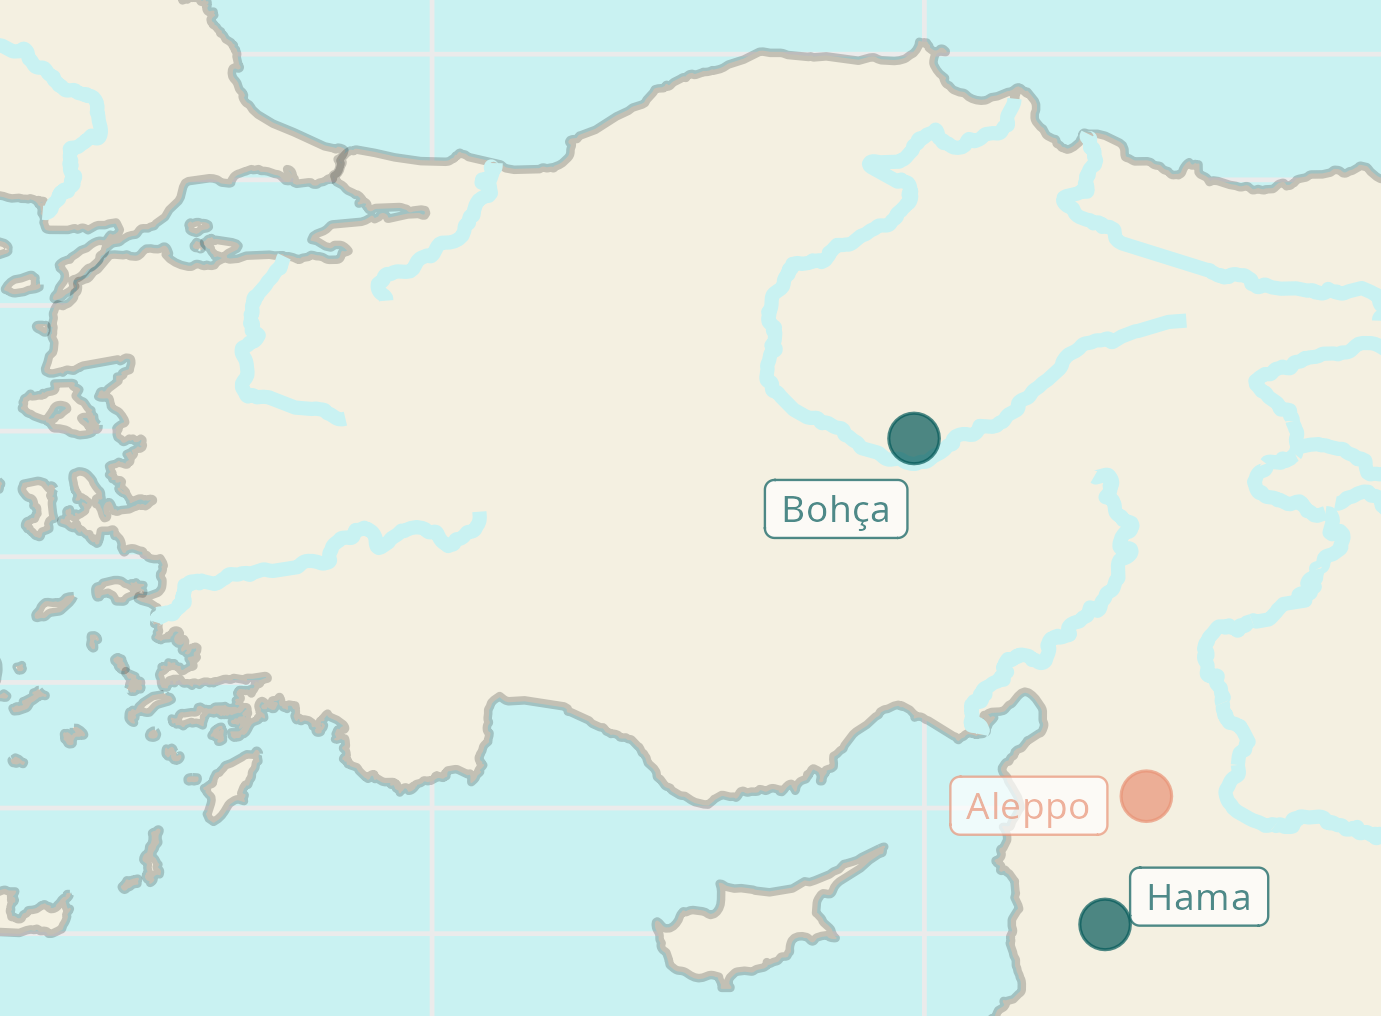
\includegraphics[width=0.65\textwidth]{../../../Mídia/Map03.png}
\end{center}


\begin{figure}[h]
	\centering
	\begin{subfigure}{0.49\textwidth}
		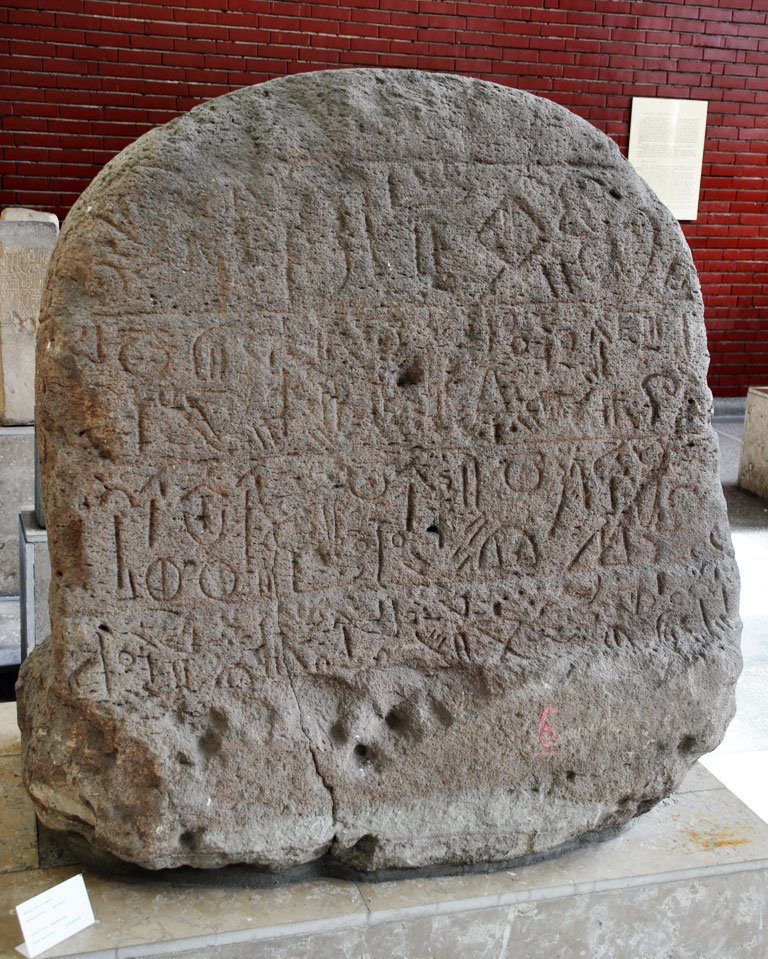
\includegraphics[width=0.9\textwidth]{../../../Mídia/bahce08.jpg}
	\end{subfigure}
	\hfill
	\begin{subfigure}{0.49\textwidth}
		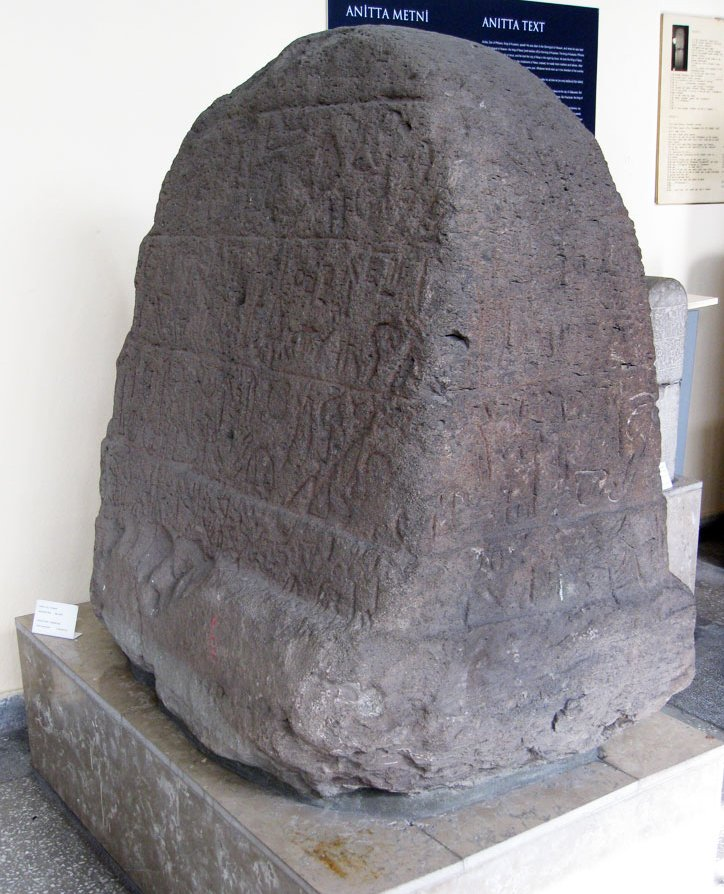
\includegraphics[width=0.9\textwidth]{../../../Mídia/bahce10.jpg}
	\end{subfigure}
	\caption[BOHÇA]{Inscrição BOHÇA. Dimensões da inscrição:
		1.26\times0.63m.
		Imagens de Cüneyt Süer, 2011,
		disponíveis em
		\href{https://www.hittitemonuments.com/bahcekoy/}{Hittite Monuments}.
		Edição e traçado em~\citeabbrev*{CHLI11}, pp.\ 478ff.\ e \emph{plate}
		265.
	}\label{fig:bohça}
\end{figure}

\clearpage

\begin{center}
	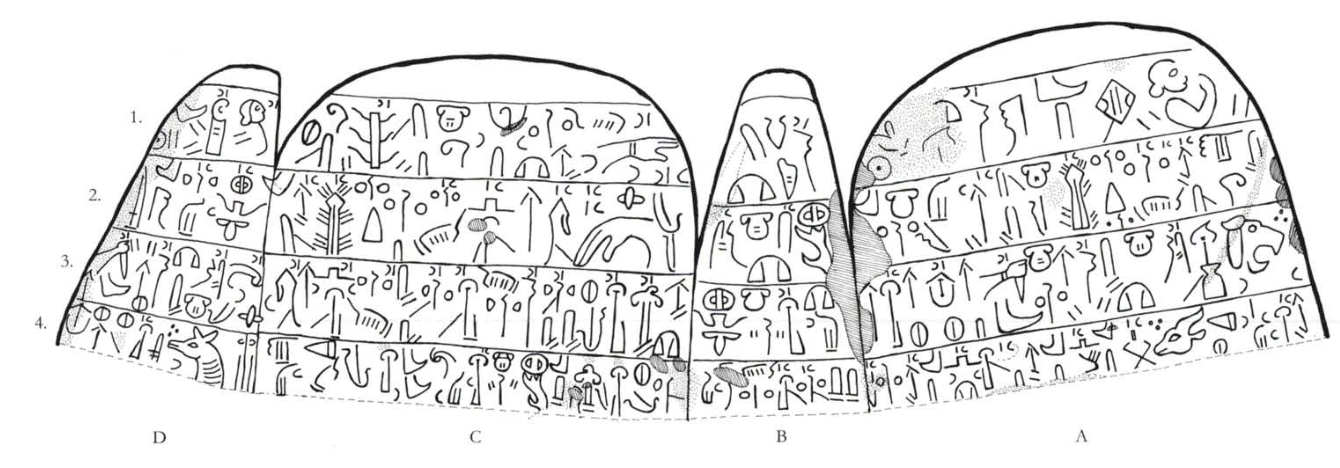
\includegraphics[width=\textheight,angle=90]{../../../Mídia/bohça.png}
\end{center}



\clearpage
\begin{parnumbersa}[]
	\raggedright%

	\Large \luwiantrans{EGO-mi}\hspace{5pt}
	[\luwmasc]\luwiantrans{ku-ra-ti-i-sá}\hspace{5pt}
	\luwmasc\luwiantrans{á-[sa-hwi-si]-sa4}\hspace{5pt}
	\luwmasc\luwiantrans{HEROS-li-i-sa}\hspace{5pt}
	\luwmasc\luwiantrans{<FILIUS>-ni-mu-wi-za-sa}\hspace{5pt}
	\luwiantrans{<OCCIDENS>-i-pa-ma-i+ri-i}\hspace{5pt}
	\luwmasc\luwiantrans{ORIENS-mi-ma-i+ri-ha}\hspace{5pt}
	\luwmasc\luwiantrans{PRAE}\hspace{5pt}
	\luwmasc\luwiantrans{AUDIREMI-ti-mi-sa4}\hspace{5pt}
	[\luwmasc]\luwiantrans{REX-ti-sá}\hspace{5pt}

	\Large \luwmasc\luwiantrans{wa-ta}\hspace{5pt}
	\luwmasc\luwiantrans{DEUS-TONITRUS-hu-ti}\hspace{5pt}
	\luwmasc\luwiantrans{za-i+ri}\hspace{5pt}
	\luwmasc\luwiantrans{BONUS-wa-su-wa-i}


	\Large \luwmasc\luwiantrans{wa-mu}\hspace{5pt}
	\luwmasc\luwiantrans{TERRA-REL-ra-zi}\hspace{5pt}
	\luwmasc\luwiantrans{SUPER-ra}\hspace{5pt}
	\luwmasc\luwiantrans{<CAPERE>-lu-na-'}\hspace{5pt}
	\luwmasc\luwiantrans{pi-pa-sa-i}\hspace{5pt}


	\Large \luwmasc\luwiantrans{DEUS-CERVUS3-ti-pa-wa-ta-'}\hspace{5pt}
	\luwmasc\luwiantrans{za-i+ri-ia-pa-a}\hspace{5pt}
	\luwmasc\luwiantrans{BONUS-wa-su-wa-i}


	\Large\luwmasc\luwiantrans{wa-mu}\hspace{5pt}
	\luwmasc\luwiantrans{za-ri+i}\hspace{5pt}
	\luwmasc\luwiantrans{sà-ma-ia}\hspace{5pt}
	\luwmasc\luwiantrans{<ANIMA-LEO>-hwi-sa5-ra}\hspace{5pt}
	\luwmasc\luwiantrans{pi-pa-sa-ia}


	\Large\luwmasc\luwiantrans{á-mi-zi-pa-wa}\hspace{5pt}
	\luwmasc\luwiantrans{tá-ti-zi-i}\hspace{5pt}
	\luwmasc\luwiantrans{AVUS-ha-zi-ha}\hspace{5pt}
	\luwmasc\luwiantrans{REL-zi}\hspace{5pt}
	[\luwmasc]\luwiantrans{sa-ta}\hspace{5pt}


	\Large\luwmasc\luwiantrans{REL-pa-wa}\hspace{5pt}
	\luwiantrans{DEUS-TONITRUS-hu-za-sa}\hspace{5pt}
	\luwmasc\luwiantrans{NEG2}\hspace{5pt}
	\luwmasc\luwiantrans{REL-ha-na}\hspace{5pt}
	\luwmasc\luwiantrans{wa-ra-ia-ia}\hspace{5pt}


	\Large\luwmasc\luwiantrans{á-mu=wa}\hspace{5pt}
	\luwmasc\luwiantrans{REL-ra}\hspace{5pt}
	\luwmasc\luwiantrans{wa-ra-ia-ia}\hspace{5pt}



\end{parnumbersa}

\vspace{10pt}
\hrule
\vspace{10pt}

\setcounter{parcount}{0}
\begin{parnumbersa}[]

	\raggedright%
	\itshape%

	\logo{EGO}-mi
	$[$\lmasc\textsuperscript{?}$]$ku+ra/i-ti-i-sá
	\lmasc{}á-[sa-hwi/a-si]-sa\textsubscript{4}
	\lmasc{}\logo{HEROS}-li-i-sa
	\lmasc{}\logo{``FILIUS''}-ni-mu-wa/i-za-sa
	\logo{``OCCIDENS''}i-pa-ma-ri+i-i
	\lmasc{}\logo{ORIENS}+MI-ma-ri+i-ha
	\lmasc{}\logo{PRAE}
	\lmasc{}\logo{AUDIRE}+MI-ti-mi-[sa\textsubscript{4}]
	\lbreak{} $[$\lmasc$]$\logo{REX}-ti-sá


	\lmasc{}wa/i-ta
	\lmasc{}\logo{DEUS.TONITRUS}-hu-ti
	\lmasc{}za-ri+i
	\lmasc{}BONUS-wa/i-su-wa/i-i


	\lmasc{}wa/i-mu
	\lmasc{}\logo{TERRA}-kwi+ra/i-zi
	\lmasc{}\logo{SUPER}+ra/i
	\lmasc{}\logo{``CAPERE''{(-)}}lu/a/i-na-'
	\lmasc{}pi-pa-sa-i


	\lmasc\logo{DEUS.CERVUS\textsubscript{3}}-ti-pa-wa/i-ta-'
	\lmasc{}za-ri+i{(-)}ia{(-)}pa-a
	\lmasc\logo{BONUS}-wa/i-su-wa/i-i


	\lmasc{}wa/i-mu
	\lmasc{}za-ri+i
	\lmasc{}sà-ma-ia
	\lbreak{}\lmasc{}\logo{``ANIMA.LEO''}-hwi/a-sa\textsubscript{5}+ra/i
	\lmasc{}pi-pa-sa-ia


	\lmasc{}á-mi-zi-pa-wa/i
	\lmasc{}tá-ti-zi-i
	\lmasc\logo{AVUS}-ha-zi-ha
	\lmasc{}\logo{REL}-zi
	$[$\lmasc\textsuperscript{?}$]$sa-ta


	\lmasc{}\logo{REL}-pa-wa/i \logo{DEUS.TONITRUS}-hu-za-sa
	\lmasc{}\logo{NEG\textsubscript{2}}
	\lmasc{}\logo{REL}-ha-na
	\lmasc{}wa/i+ra/i-ia-ia


	\lmasc{}á-mu-wa/i
	\lmasc{}\logo{REL}+ra/i
	\lmasc{}wa/i+ra/i-ia-ia



\end{parnumbersa}

\vspace{10pt}
\hrule
\vspace{10pt}


\setcounter{parcount}{0}
\begin{parnumbersa}[]

	\raggedright%
	\itshape%

	amu=mi Kurtis, Ashwisis \logo{HEROS}-lis nimuwizas,
	ipamari kistamari=ha paran tumantimis hantawatis.

	*a=wa=ta Tarhunti zari wasuwi,

	*a=wa=mu taskwirinzi sara luna pipasai.

	Runt{(iy)}i=pa=wa=ta zari {??} wasuwi,

	*a=wa=mu zari samaya hwisara pipasaya.

	aminzi=pa=wa tatinzi huhanzi=ha kwinzi *asata,

	kwipa=wa Tarhunzas na kwishan wariyaya,

	amu=wa kwari wariyaya:


\end{parnumbersa}

\vspace{10pt}
\hrule
\clearpage



\begin{parnumbersa}[]
	\raggedright%

	\Large\luwmasc\luwiantrans{wa-mu}\hspace{5pt}
	\luwmasc\luwiantrans{TERRA-REL-ra-zi}\hspace{5pt}
	\luwmasc\luwiantrans{SUPER-ra}\hspace{5pt}
	\luwmasc\luwiantrans{<CAPERE>-lu-na-'}\hspace{5pt}
	\luwmasc\luwiantrans{pi-pa-sa-i}\hspace{5pt}


	\Large \luwiantrans{á-mi-zi-ha-[wa]}\hspace{5pt}
	\luwmasc\luwiantrans{tá-ti-zi}\hspace{5pt}
	\luwiantrans{AVUS-ha-zi-ha[-']}\hspace{5pt}
	\luwmasc\luwiantrans{REL-i}\hspace{5pt}
	\luwiantrans{<ANIMA.EQUUS[>]-zú-sà-ta-la-u-na}\hspace{5pt}
	\luwmasc\luwiantrans{REL}\hspace{5pt}
	\luwmasc\luwiantrans{<PES2PES2>-da-ta}


	\Large\luwmasc\luwiantrans{REL-pa-wa}\hspace{5pt}
	\luwiantrans{DEUS-CERVUS3-ti-ia-[sá]}\hspace{5pt}
	[\luwmasc]\luwiantrans{NEG2-a}\hspace{5pt}
	[\luwmasc]\luwiantrans{REL-ha-na}\hspace{5pt}
	\luwmasc\luwiantrans{wa-ra-[ia]-ta}\hspace{5pt}


	\Large[\luwmasc]\luwiantrans{á-mu-wa}\hspace{5pt}
	\luwmasc\luwiantrans{REL-ra}\hspace{5pt}
	\luwmasc\luwiantrans{wa-ra-ia-ia}\hspace{5pt}


	\Large[\luwmasc]\luwiantrans{[a]-wa}\hspace{5pt}
	\luwmasc\luwiantrans{za-ti-i}\hspace{5pt}
	\luwmasc\luwiantrans{TERRA-sa-REL-ra-i}\hspace{5pt}
	\luwmasc\luwiantrans{za-ti-i}\hspace{5pt}
	\luwmasc\luwiantrans{LOCUS-lá-ti-i}\hspace{5pt}
	\luwiantrans{1 CENTUM}\hspace{5pt}
	\luwiantrans{ANIMA-CAPRA}\hspace{5pt}
	\luwmasc\luwiantrans{la-ha}\hspace{5pt}
	\luwmasc\luwiantrans{<UNUS>-ta}\hspace{5pt}
	\luwmasc\luwiantrans{REL-za}\hspace{5pt}



\end{parnumbersa}

\vspace{10pt}
\hrule
\vspace{10pt}

\setcounter{parcount}{8}
\begin{parnumbersa}[]

	\raggedright%
	\itshape%

	\lmasc{}wa/i-mu
	\lmasc{}\logo{“TERRA”}-kwi+ra/i-zi \logo{SUPER}+ra/i
	\lmasc{}\logo{“CAPERE”}{(-)}lu\logo/a/i-na
	\lmasc{}pi-pa-sa-ia


	\lmasc{}á-mi-zi-ha<-wa/i>
	\lmasc{}tá-ti-zi
	\lbreak{} \logo{AVUS}-ha-zi-ha-a?
	\lmasc{}\logo{REL}-i
	\logo{“ANIMA.EQUUS<”>}-zú-sà-ta-la-u-na
	\logo{REL}
	\logo{“PES\textsubscript{2}.PES\textsubscript{2}”}{(-)}da-ta


	\lmasc{}\logo{REL}-pa-wa/i
	\logo{DEUS.CERVUS\textsubscript{3}}-ti-ia-\textsc{⌈}sá\textsuperscript{?}\textsc{⌉} $[$\lmasc{}\textsuperscript{?}$]$\logo{NEG\textsubscript{2}}-a
	$[$\lmasc{}\textsuperscript{?}$]$\logo{REL}-ha-na
	$[$\lmasc{}\textsuperscript{?}$]$wa/i+ra/i-[ia?]-ta

	$[$\lmasc{}\textsuperscript{?}$]$á-mu-wa/i
	\lmasc{}\logo{REL}+ra/i
	\lmasc{}wa/i+ra/i-ia-ia


	\lmasc{}\textsc{⌈}a\textsuperscript{?}\textsc{⌉}-wa/i
	\lmasc{}za-ti-i
	\lmasc{}\logo{“TERRA”}-sa-kwi+ra/i-i
	\lmasc{}za-ti-i
	\lmasc{}\logo{LOCUS}-lá/í-ti-i \logo{1\times{}CENTUM} \logo{ANIMA.CAPRA} la-ha
	\logo{“UNUS”}-ta
	\lmasc{}\logo{REL}-za


\end{parnumbersa}

\vspace{10pt}
\hrule
\vspace{10pt}


\setcounter{parcount}{8}
\begin{parnumbersa}[]

	\raggedright%
	\itshape%

	*a=wa=mu taskwirinzi sara luna pipasai

	aminzi=ha=wa tatinzi huhanzi=ha kwi azusataluna {??}
	\logo{PES\textsubscript{2}.PES\textsubscript{2}}-danta,

	kwipa=wa Runtiyas na kwishan wariyata.

	amu=wa kwari wariyaya

	a=wa zadi taskwiri zadi \logo{LOCUS}-lati $100$ sasanzi laha \logo{UNUS}-ta kwanza \ldots{}

\end{parnumbersa}

\vspace{10pt}
\hrule

\clearpage
\begin{multicols}{2}[\noindent\textbf{Vocabulário}]
	\begin{hangparas}{1em}{1}
		\raggedright%
		\textbf{\emph{Ashwisi}-} (NP) \tabto{1em} Ashwisis\\
		\textbf{\emph{azusatala}-} (\emph{v.i.}) \tabto{1em} andar a cavalo, cavalgar\\
		\textbf{\emph{\emph{HERO}-li}-} (NP) \tabto{1em} herói\\
		\textbf{\emph{huha}-} (\emph{subst.com.}) \tabto{1em} avô\\
		\textbf{\emph{hwisar}-} (\emph{subst.neut.}) \tabto{1em} fera, animal selvagem\\
		\textbf{\emph{ipami}-} (\emph{subst.com.}) \tabto{1em} ocidente\\
		\textbf{\emph{kistami}-} (\emph{subst.com.}) \tabto{1em} oriente\\
		\textbf{\emph{Kurti}-} (NP) \tabto{1em} Kurtis\\
		\textbf{\emph{kwi}} (\emph{adv.}) \tabto{1em} quando\\
		\textbf{\emph{kwipa}} (\emph{adv.}) \tabto{1em} de fato\\
		\textbf{\emph{la}-} (\emph{v.t.}) \tabto{1em} tomar\\
		\textbf{\emph{\emph{LOCUS}-la}- = \emph{arla}-?} (\emph{subst.neut.}) \tabto{1em} lugar\\
		\textbf{\emph{na kwishan}} (\emph{adv.}) \tabto{1em} de modo algum\\
		\textbf{\emph{paran tumanti}-} (\emph{v.t.}) \tabto{1em} ouvir falar de\\
		\textbf{\emph{\emph{PES\textsubscript{2}.PES\textsubscript{2}}-da}-} (\emph{v.i.}) \tabto{1em} ir fazer + \textsc{Inf.}\\
		\textbf{pipasa-} (\emph{v.t.}) \tabto{1em} permitir (\emph{iter.} \emph{pi{(ya)}-} `dar')\\
		\textbf{\emph{sasa}-} (\emph{subst.com.}) \tabto{1em} cabra? bode?\\
		\textbf{\emph{taskwira}-} (\emph{subst.com.}) \tabto{1em} terra, território\\
		\textbf{\emph{tati}-} (\emph{subst.com.}) \tabto{1em} pai\\
		\textbf{\emph{tumanti}-} (\emph{v.t.}) \tabto{1em} ouvir\\
		\textbf{\emph{\emph{UNUS}-ta}} (\emph{adv.}) \tabto{1em} de uma vez\\
		\textbf{\emph{wariya}-} (\emph{v.t.}) \tabto{1em} ajudar\\
		\textbf{\emph{wasu-}} (\emph{v.t.}) \tabto{1em} ser bom para + \Dat{}\\
		\textbf{\emph{zadi}} (\emph{adv.}) \tabto{1em} aqui\\
	\end{hangparas}
\end{multicols}

\subsubsection*{Notas}

\paragraph{1}
\textbf{amu=mi} `eu (sou)': o verbo \emph{as-} `ser, estar' é com frequência deixado
explícito em sentenças nominais e nestes casos costuma-se utilizar a
forma reflexiva do pronome.

\paragraph{5}
\textbf{samaya} `?': há três interpretações para o termo:
\begin{inparaenum}
	\item a palavra é um substantivo neutro plural, agindo como aposto de
	\emph{hwisara} `animais selvagens, feras' e está associada a
	\emph{samanza} `selos' (KULULU 2, §2), talvez um substantivo derivado do
	verbo \emph{sa-} `selar, imprimir',
	dando o sentido de `ele me concede as feras, o combinado'.
	\item a palavra é um substantivo dativo singular, possivelmente derivado do
	mesmo verbo \emph{sa-} `selar, imprimir' com o sentido associado de
	`marcar $\rightarrow$ atirar, ferir', dando o sentido de `ele me deu as
	feras para ferir\slash{}atirar'.
	\item a palavra é um adjetivo concordando com \emph{hwisara}, sem sentido
	conhecido, talvez um plural neutro de \emph{sami-} `atirado, ferido'.
\end{inparaenum}

\bigskip
\noindent \textbf{Tradução}\\
\noindent [1] Eu sou Kurtis, filho do herói Ashwisis, rei conhecido do
pelo ocidente e oriente.

\noindent [2] Aqui eu sou bom para Tarhunta [3] e ele me
permite tomar (os) territórios.
[4] E aqui eu sou bom para Runtiya [5] e ele me concede (as) feras SAMAYA\@.

\noindent [6] Àqueles que foram meus pais e avôs [7] de fato Tarhunta não
ajuda de modo algum, [8] como ele me ajuda: [9] ele me permite tomar (os)
territórios.

\noindent [10] E quando meus pais e avôs iam cavalgar, [11] de fato Runtiya não
os ajudou de modo algum, [12] como ele me ajuda: [13] aqui em (seu) território,
aqui em (seu) lugar, capturei cem gazelas de uma vez \ldots



\backmatter%

\printbibliography%


\end{document}
